%\documentclass[a4paper]{article}
\usepackage[utf8]{inputenc}
\usepackage[spanish, es-tabla, es-noshorthands]{babel}
\usepackage[table,xcdraw]{xcolor}
\usepackage[a4paper, footnotesep=1.25cm, headheight=1.25cm, top=2.54cm, left=2.54cm, bottom=2.54cm, right=2.54cm]{geometry}
%\geometry{showframe}

%\usepackage{wrapfig}			%Wrap figure in text
\usepackage[export]{adjustbox}	%Move images
\usepackage{changepage}			%Move tables

\usepackage{tikz}
\usepackage{amsmath}
\usepackage{amsfonts}
\usepackage{amssymb}
\usepackage{float}
\usepackage{graphicx}
\usepackage{caption}
\usepackage{subcaption}
\usepackage{multicol}
\usepackage{multirow}
\usepackage{wrapfig}
\setlength{\doublerulesep}{\arrayrulewidth}
\usepackage{booktabs}
\usepackage[numbib, nottoc, notlot, notlof]{tocbibind}

\usepackage{hyperref}
\hypersetup{
    colorlinks=true,
    linkcolor=blue,
    filecolor=magenta,      
    urlcolor=blue,
    citecolor=blue,    
}

%Change Font Size

% #1 = size, #2 = text
\newcommand{\setparagraphsize}[2]{{\fontsize{#1}{6}\selectfont#2 \par}}		%Cambia el size de todo el parrafo
\newcommand{\setlinesize}[2]{{\fontsize{#1}{6}\selectfont#2}}				%Cambia el font de una oración

\newcommand{\note}[1]{
	\begin{center}
		\huge{ \textcolor{red}{#1} }
	\end{center}
}

%FONTS (IMPORTANTE): Compilar en XeLaTex o LuaLaTeX
\usepackage{anyfontsize}	%Font size
\usepackage{fontspec}		%Font type

\usepackage{etoolbox}
\usepackage{todonotes}

\newcommand{\observacion}[2]{  \ifnumequal{1}{#1}{ { \todo[inline,backgroundcolor=red!25,bordercolor=red!100]{\textbf{Observación: #2}} } }{  }  }

\setcounter{topnumber}{2}
\setcounter{bottomnumber}{2}
\setcounter{totalnumber}{4}
\renewcommand{\topfraction}{0.85}
\renewcommand{\bottomfraction}{0.85}
\renewcommand{\textfraction}{0.15}
\renewcommand{\floatpagefraction}{0.8}
\renewcommand{\textfraction}{0.1}
\setlength{\floatsep}{5pt plus 2pt minus 2pt}
\setlength{\textfloatsep}{5pt plus 2pt minus 2pt}
\setlength{\intextsep}{5pt plus 2pt minus 2pt}

\newcommand{\quotes}[1]{``#1''}
\usepackage{array}
\newcolumntype{C}[1]{>{\centering\let\newline\\\arraybackslash\hspace{0pt}}m{#1}}
\usepackage[american]{circuitikz}
\usetikzlibrary{calc}
\usepackage{fancyhdr}
\usepackage{units} 

\graphicspath{{../Control de posición no lineal/}{../Control de fuerza no lineal/}{../Control híbrido no lineal/}{../Referencias/}{../Deducción de modelo/}{../Conclusiones/}}

\pagestyle{fancy}
\fancyhf{}
\lhead{22.99 - Automación Industrial}
\rhead{Lambertucci, Londero B., Maselli, Mechoulam}
\rfoot{Página \thepage}

%Items con bullets y no cuadrados
\renewcommand{\labelitemi}{\textbullet }

%
%\begin{document}

\Subsection{Modelo de Simscape}
\label{sec:simulacionessimscape}
Para lograr mayor apego a la realidad, se decidió utilizar un modelo con fricción obtenido utilizando el framework de Simscape de Simulink, que se pueden observar en las Figuras (\ref{fig:simscape}) y (\ref{fig:simscape_dp}).

Los valores de fricción que se utilizaron para cada joint son de $0.004 \ \frac{N\cdot s}{m}$, resultando así en las siguientes matrices:

\begin{equation}
 A_{simscape} = \begin{bmatrix}
0 &  0 & 0 & 1 &  0 & 0\\
0 &  0 & 0 & 0 &  1 & 0\\
0 &  0 & 0 & 0 &  0 & 1\\
0 &  -3.1784 & 0.3973 & -0.0008 &  0.0557 & -0.0681\\
0 &  16.6865 & -13.1108 & 0.001 &  -0.4646 & 0.8734\\
0 &  -20.3946 & 35.6243 & -0.0012 &  0.8734 & -1.9842
\end{bmatrix}
\end{equation}
\begin{equation}
 B_{simscape} = \begin{bmatrix}
0 \\
0 \\
0 \\
0.1892 \\
-0.2432 \\
0.2973 
\end{bmatrix}
\end{equation}

de ahora en más llamadas simplemente A y B. Estas matrices son muy similares a las obtenidas teóricamente, con la excepción más notoria del corrimiento de uno de los dos polos en el origen hacia el semiplano izquierdo.

\begin{figure}[H]
	\centering
	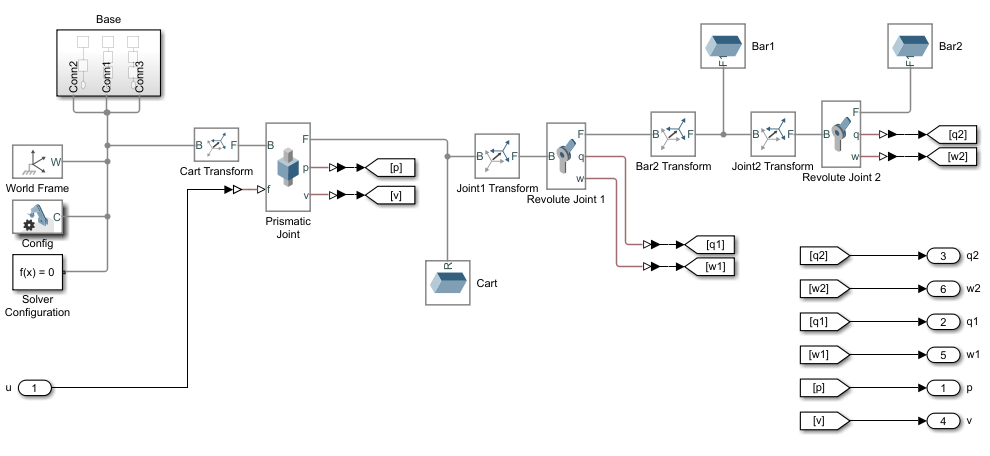
\includegraphics[width=1\linewidth]{../Simulaciones/ImagenesSimulaciones/simscape.png}
	\caption{Bloques de la simulación del péndulo doble realizada con el framework de Simscape en Simulink.}	
	\label{fig:simscape}
\end{figure}
\begin{figure}[H]
	\centering
	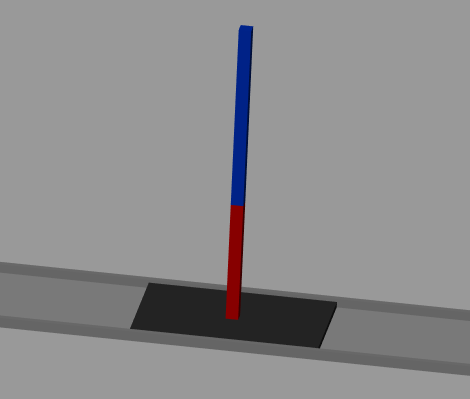
\includegraphics[width=0.7\linewidth]{../Simulaciones/ImagenesSimulaciones/simscape_double_pendulum.png}
	\caption{Simulación del péndulo doble realizada con el framework de Simscape en Simulink.}	
	\label{fig:simscape_dp}
\end{figure}

\Subsection{Simulink}
%\end{document}